
\catalin{Explain the code in more detail. Also mention the interrupt part for gpio.}
\subsection{CAN Controller Software}
\subsubsection{Implementation in code}~\\
As mentioned in section \ref{sub:Basic_SourceCode}, the code was based on the xcanps polled example available by Xilinx documentation.
The important functionalities that needed to be provided by the final software version included:
\begin{itemize}
\item receiving and sending of frames
\item creating the message id
\item decoding of the message id parts, such as the node id, the message type etc. \catalin{what else?}
\item handling button interrupts
\item controlling the LEDs
\item accepting and ignoring messages according to the subscriptions list
\end{itemize}
\catalin{What other functionalities? And, 1st letters capitals or not?}
The figure \ref{fig:SeqDiagram_SendFrame} shows the procedure of sending a frame to the CAN network containing data, which makes use of the protocol function createMsgID().
After returning the message id, the id and the data are put into the TxFrame to be sent once the FIFO has space.
The actual sending is done with a call to the XCanPs function XCanPs\_Send().
\\
Similarly, the procedure of receiving a frame is shown in the figure \ref{fig:SeqDiagram_RecvFrame}.
The node once it calls the RecvFrame() function, it waits in a loop until it receives a frame. Then, it checks the subscriptions in order to forward the packet for further processing or to ignore it.


This was achieved by implementing a set of functions and an array variable of subscriptions for each node.

\begin{figure}[h!]
	\centering
	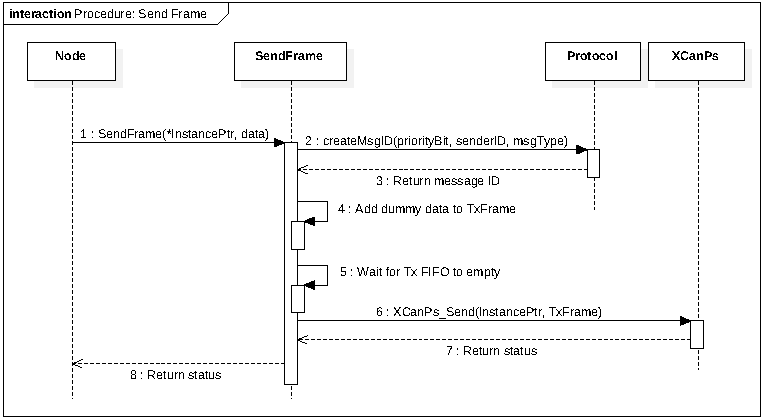
\includegraphics[width = 1.1\linewidth]{graphics/SeqDiagram_SendFrame.pdf}
	\caption{The sequence diagram of the process of sending a frame.}
	\label{fig:SeqDiagram_SendFrame}
\end{figure}

\begin{figure}[h!]
	\centering
	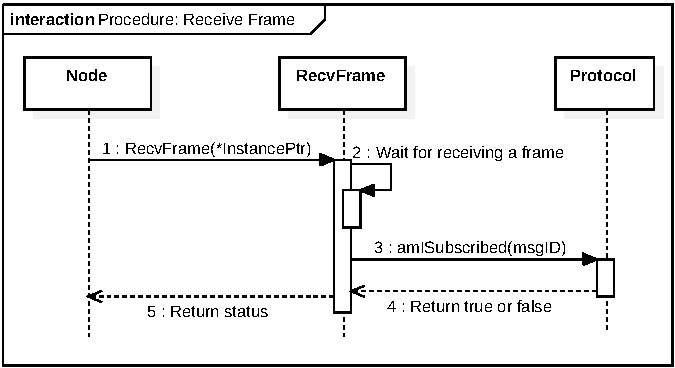
\includegraphics[width = 1.1\linewidth]{graphics/SeqDiagram_RecvFrame.pdf}
	\caption{The sequence diagram of the process of receiving a frame.}
	\label{fig:SeqDiagram_RecvFrame}
\end{figure}

\begin{figure}[h!]
	\centering
	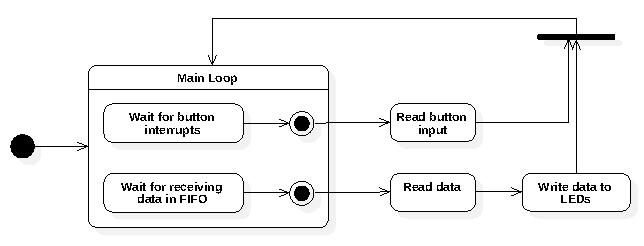
\includegraphics[width = 1.1\linewidth]{graphics/StateDiagram_CanStackTestCode.pdf}
	\caption{Behavioral diagram of the basic source code.}
	\label{fig:CAN_Testing_StateDiagr_Code}
\end{figure}